\chapter{Systementwurf}


\section{Abtastung}
Idee ist es, das aufgenommene Bild in vier verschiedene Regionen einzuteilen. (Siehe Bild \ref{fig:Regions})

\begin{figure}[hb]
	\centering
	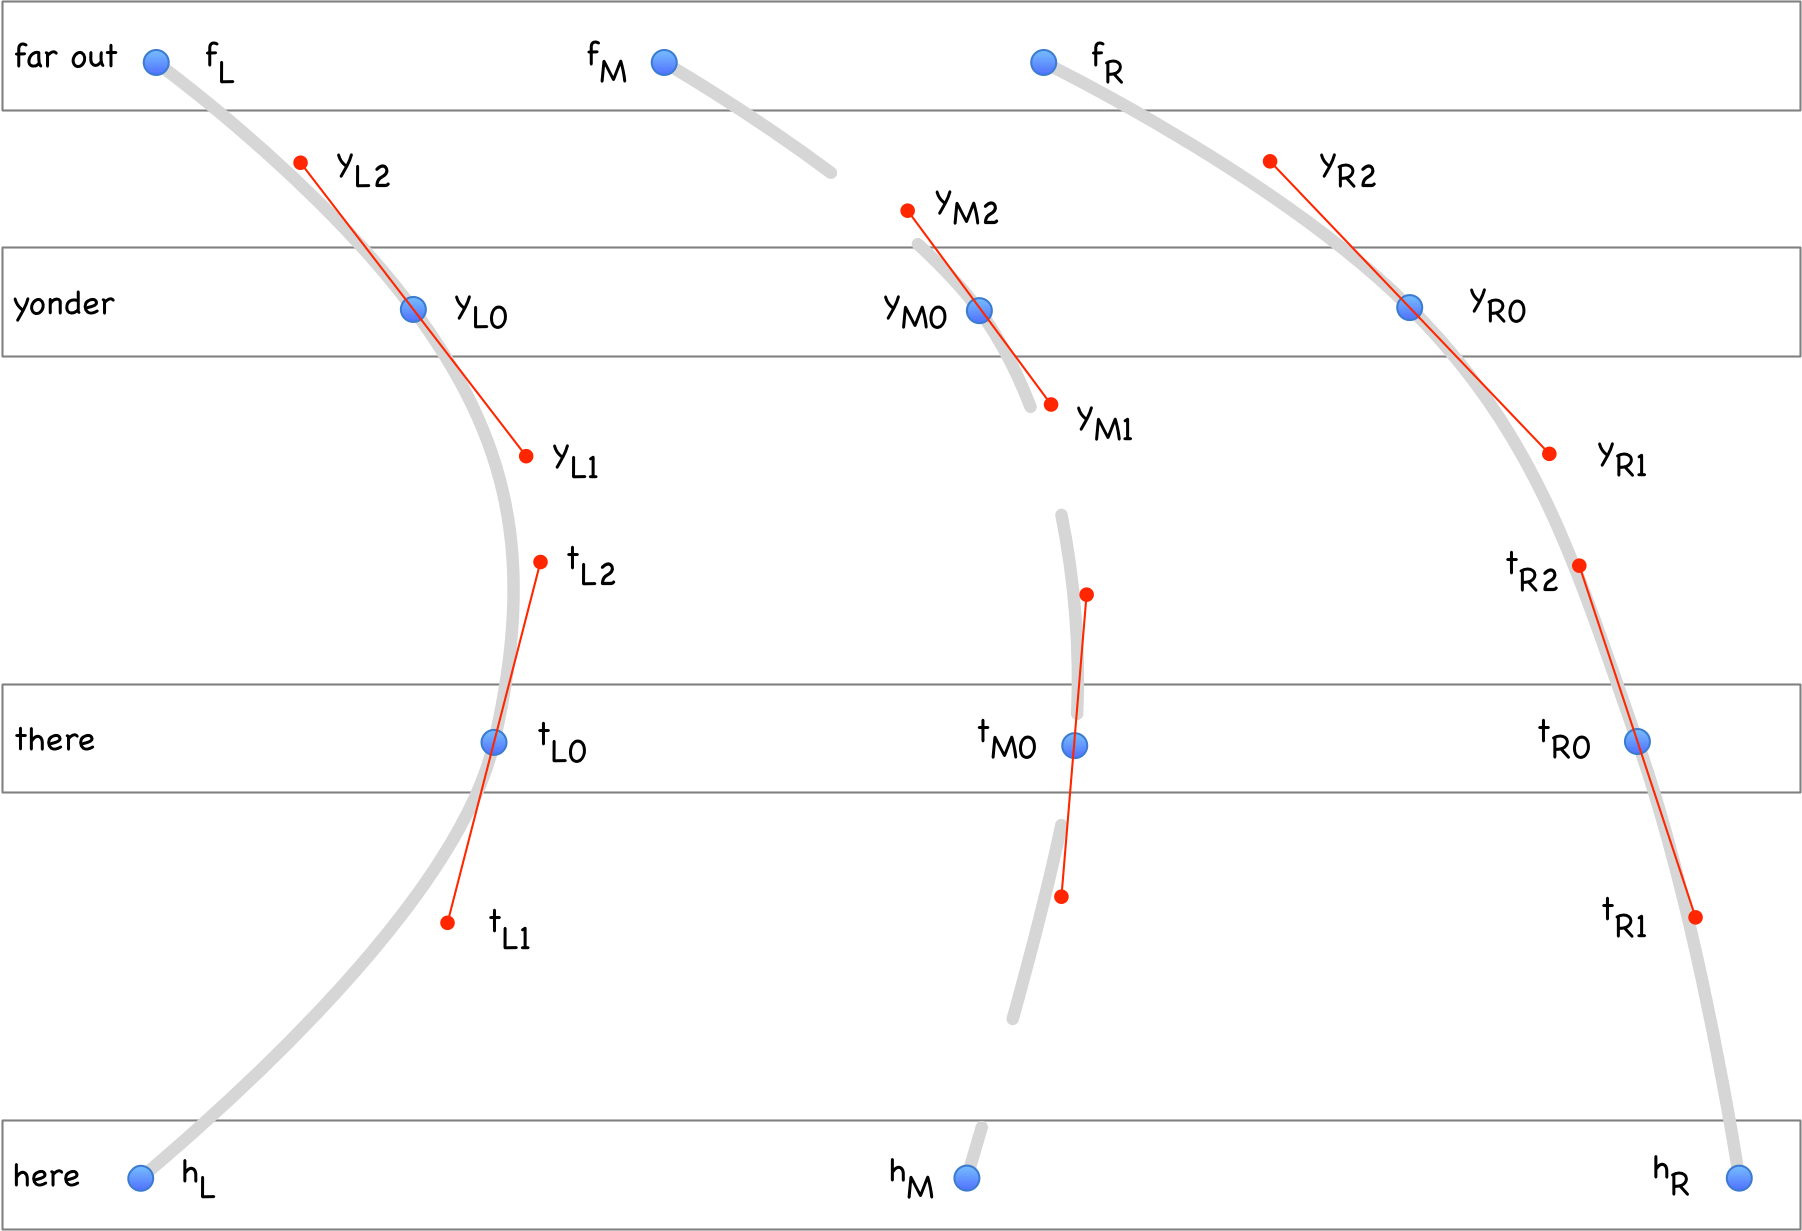
\includegraphics[scale=0.5]{bilder/SA/Sc-full.png}
	\caption{Verschiedene Regionen}
	\label{fig:Regions}
\end{figure}

\newpage

F�r jede dieser Regionen wird jeweils eine Zeile abgetastet. Als Ergebnis erh�lt man ein Histogram (Siehe Bild \ref{fig:Regions}). Man kann erkennen, dass die Spurmarkierungen durch Peaks mit einer bestimmten Breite und einem bestimmten Abstand (in Gr�n) zueinander erkennbar sind.
In Rot zu erkennen sind Artefakte, welche sich durch eine kleine Breite(1-2px) auszeichnen.
Sie entstehen zum Beispiel durch Reflexionen auf der Fahrbahn.

\begin{figure}[hb]
	\centering
	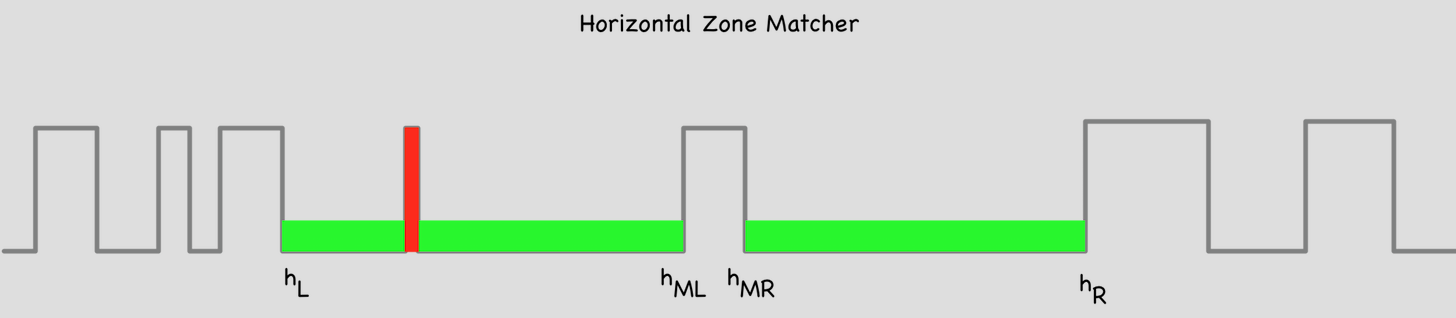
\includegraphics[scale=0.6]{bilder/SA/Histogramm.png}
	\caption{Histogramm}
	\label{fig:Histogramm}
\end{figure}

\subsection{Eleminiere Artefakte}
Um Artefakte und Objekte ohne Kante zu eliminieren werden die abgetasteten Regionen mit der Canny Kantenerkennung gefiltert. �brig bleiben Punkte, die zu einer Kante geh�ren und deutlich weniger Artefakte.



\section{Wahrscheinlichkeitsverteilung}

F�r jeden gefunden Punkt in der Region soll bestimmt werden mit welcher Wahrscheinlichkeit dieser zu einer Spurmarkierung der rechten Fahrspur geh�rt. Verschiedene Filter werden daf�r eingesetzt, jeder dieser Filter addiert eine Wahrscheinlichkeit zu jedem der gefundenen Punkte.
Initial erhalten alle Punkte die Wahrscheinlichkeit null.

\subsection{Filter ROI}

\subsection{Filter Spurbreite}

\subsection{Filter Streifenbreite}

\subsection{Filter Tiefpass}

\subsection{Trafo}

\section{Szenarien}

\subsection{Ausbleibende Spur}
\subsubsection{Verhalten}

\subsection{Zebrastreifen}
\subsubsection{Zebrastreifen Erkennung}
\subsubsection{Verhalten}

\subsection{Kreuzung}
\subsubsection{Stopplinien Erkennung}
\subsubsection{Verhalten}

\subsection{Weitere denkbare Szenarien}

\section{Ausblick}

\subsection{Vortasten}

\subsection{Kalman Filter}















